\chapter{Theorie}

\section{Grundlagen MRT}
Die Magnetresonanztomographie (MRT) ist ein Bildgebendes Verfahren, bei der keine ionisierender Strahlung eingesetzt wird.
Dadurch gibt es keine Strahlenbelastung für Patientinnen und Patienten und die Untersuchung kann beliebig oft wiederholt werden.
Die MRT wird zur Darstellung von morphologischen Strukturen und zur Abbildung funktioneller Prozesse verwendet.
Das MRT-Gerät besteht aus einem zylinderförmigen, supraleitenden Magneten, der ein homogenes Hauptmagnetfeld $B_0$ erzeugt. %Shimming optional
In der klinischen Anwendung liegt die Magnetfeldstärke bei $\qty{1.5}{T}$ - $\qty{3}{T}$.~\cite{Schlegel}
Die Kernteilchen besitzen einen magnetischen Moment $\vec{m}$, aufgrund dessen das sie um ihre eigene Achse, mit der Lamorfrequenz 
\begin{equation}
    \omega_0 = \gamma \cdot B_0
\end{equation}
präzedieren. $\gamma$ beschriebt dabei das Gyromagnetische Verhältnis, welches Materialabhängig ist.
Die magnetischen Momente des Kerns summieren sich und es entsteht eine gesamt Magnetisierung $\vec{M}$ des Atoms. Befinden sich diese Atome im Magnetfeld,
richten sich die Spins der Kernteilchen parallel und antiparallel nach dem Magnetfeld aus. Sie befinden sich im thermischen Gleichgewicht.
Bei Atomen mit einer geraden Anzahl an Kernteilchen heben sich beim aufsummieren die magnetischen Momente auf und besitzen somit keine
Magnetisierung. 
Da die Magnetisierung notwendig für die Messung eines Signals im MRT ist, können nur Atome mit einer ungeraden Anzahl an Kernteilchen gemessen werden.
Am häufigsten wird zur Messung Wasserstoff verwendet, da dies mit ca. $\qty{80}{\%}$ am häufigsten im Menschlichen Körper vorkommt.
Mittels eines Hochfrequenzsignals (HF) werden die Spins um einen Winkel
\begin{equation}
    \alpha = \gamma \cdot B_1 \cdot T 
\end{equation}
gekippt. Dabei entspricht $B_1$ dem Anregungsimpuls und $T$ die Zeit des HF-Impulses.
Die Frequenz des HF-Signals entspricht der Lamorfrequenz des Atoms, damit es zur Resonanz kommt. 
Beim Ausschalten des Signals, relaxieren die Kernteilchen zurück in ihre Gleichgewichtsmagnetisierung. 
Dabei wird zwischen T1-Relaxation und T2-Relaxation unterschieden. Mittels dieser Unterscheidung und der Einstellung der Echozeit $T_E$ und 
Repetitionszeit $T_R$, sind die Bilder unterschiedlich Gewichtet.
Die Repetitionszeit beschreibt die Zeit zwischen der Verwendung zweier HF-Impulse und die Echozeit der zeitliche Abstand zwischen dem Anregungsimpuls und der Auslesung des Signals. 
Anhand der Gewichtungen entstehen unterschiedliche Kontraste.
Durch die veränderten Magnetisierung kommt es zur Induktion einer Spannung, die mittels einer Spule gemessen wird.


Bei der T1- Relaxation wird die Längsmagnetisierung betrachtet, welche mit der Zeit zunimmt.
Diese lässt sich durch 
\begin{equation}
    M_z(t) = M_z(0) (1 - e^{-\frac{t}{T_1}})
\end{equation}
% Bild 
Zur Messung des Signals, wird der Zeitpunkt $T_1$, nach der Anregung bestimmt, bei dem $\qty{63}{\%}$ der Magnetisierung wiederhergestellt wurde.~\cite{Pollmann}\\
Bei der T1 Gewichtung, sind $T_R$ und $T_E$ kurz eingestellt und zusätzlich gilt das $T_E \ll T_2$.
Fett und Muskeln werden bei dieser Gewichtung hell dargestellt und Liquor dunkel.~\cite{Schlegel}

Die T2-Relaxation beschreibt die Quermagnetisierung, welche mit der Zeit abnimmt, da die Spins dephasieren und somit das Signal zerfällt.
Dieser Signalzerfall wird als "Free Induction Decay" (FID) bezeichnet.~\cite{Dössel}
Die Magnetisierung wird durch die Formel
\begin{equation}
    M_{xy}(t) = M_{xy}(0) e^{-\frac{t}{T_2}} 
\end{equation}
beschrieben.
Zum Zeitpunkt $T_2$, wenn die transversale Magnetisierung auf $\qty{37}{\%}$ abgefallen ist, wird das Signal aufgenommen.~\cite{Pollmann}
Für T2-Gewichtete Bilder gilt, dass $T_R \gg T_1$ und sowohl $T_R$ als auch $T_E$  lang eingestellt werden. 
Bei dieser Gewichtung wird Liquor hell dargestellt und Fett und Muskeln dunkel.~\cite{Schlegel} 
Aufgrund von Inhomogenitäten im Hauptmagnetfeld, kommt es zu einem schnelleren Signalzerfall. Dies wird bezeichnet als T2* Relaxation.~\cite{Dössel}\\


Für die Erstellung des Bildes, benötigt es die drei Gradientenspulen $G_z$, $G_y$ und $G_x$. Die Anordnung der drei Spulen 
ist in Abbildung \ref{fig:an Grad} abgebildet.
\begin{figure}[htbp]
  \centering
  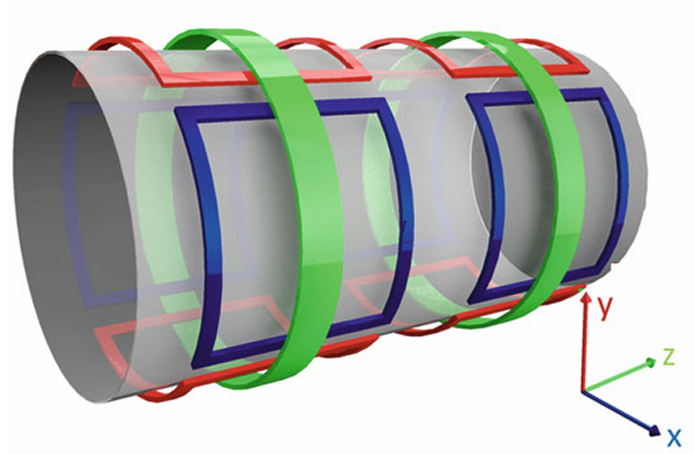
\includegraphics[scale=0.5]{/nfs/homes/sdreyer/Digit-Classification-Pytorch/tudothesis-main/content/abbildungen/Anordnung Gradientenspulen.png}
  \caption{Anordnung der Gradientenspulen.\cite{Schlegel}}
  \label{fig:an Grad}
\end{figure}
Durch das schalten der Gradienten kommt es zur Überlagerung mit dem Magnetfeld, wodurch die Codierung des Bildes möglich ist.
Der Gradient in z-Richtung wird für die Einstellung der Schichtdicke verwendet. 
Zur Frequenzcodierung wird der Gradient $G_x$ geschaltet, wodurch sich die Lamorfrequenzen entlang des Gradienten verschieben.
Mittels des Gradienten $G_y$ werden die Spins in ihrer Phase verschoben.
Durch die Verschiebung der Frequenz und Phase ist die Ortscodierung möglich und die Aufnahme eines Bildes im k-Raum.
Durch die Fouriertransformation werden die Informationen in den Ortsraum transformiert.
Dadurch liefert die MRT Bilder in Schichten, die anschließend zu einem 3D-Bild zusammengesetzt und analysiert werden.~\cite{pabst2013}


\section{Maschinelles Lernen}

Künstliche Intelligenz (KI) simuliert das Verhalten einer Menschlichen Intelligenz durch eine Maschine. 
Das Maschinelle Lernen (ML) gehört zu einem Teilbereich der Künstlichen Intelligenz. Deep Learning stellt 
wiederum einen Teilbereich des Maschinellem Lernen da. Das Deep learning beinhaltet das trainieren mehrschichtigen Neuronaler Netzwerke mit großen Datensätze.
Durch die Verwendung von Daten ist es den Algorithmen beim 
Maschinellem Lernen möglich aus diesen zu lernen und sich zu verbessern, ohne das die Algorithmen dem Problem entsprechend programmiert werden müssen.~\cite{kleesiek2020}
Somit findet das Maschinelle Lernen Anwendung in der Identifizierung und Klassifikation von Objekten, Analyse, Vorhersagen, 
Sprachverarbeitung und Informationsbeschaffung.~\cite{shinde2018}

\begin{figure}[htbp]
  \centering
  \includegraphics[scale=0.5]{/nfs/homes/sdreyer/Digit-Classification-Pytorch/tudothesis-main/content/abbildungen/Künstliche Intelligenzpng.png}
  \caption{.~\cite{kleesiek2020}}
  \label{fig:KI}
\end{figure}

Das Lernen lässt sich unterscheiden in überwachtes Lernen (Supervised Learning) und unüberwachtes Lernen (Unsupervised Learning).
Beim überwachten Lernen, sind die Eingabedaten gelabelt, sodass das Netzwerk anhand dessen lernt, indem es den Ausgabewert mit dem bekannten Zielwert 
vergleicht und das Netzwerk dementsprechend.
Beim unüberwachten Lernen erkennt der Algorithmus Muster und Strukturen in den Eingabedaten, ohne das Eingabedaten gelabelt sind.~\cite{kleesiek2020}


\subsection{Neuronales Netzwerk}

Das Neurale Netzwerk ist aufgebaut aus drei Schichten: 
Die Eingabeschicht (Input Layer), Versteckten Schichten (Hidden Layers) und die Ausgabe Schicht (Output Layer).
Der Aufbau eines Neuronalen Netzwerkes wird in der Abbildung \ref{fig:NN} dargestellt

\begin{figure}[htbp]
  \centering
  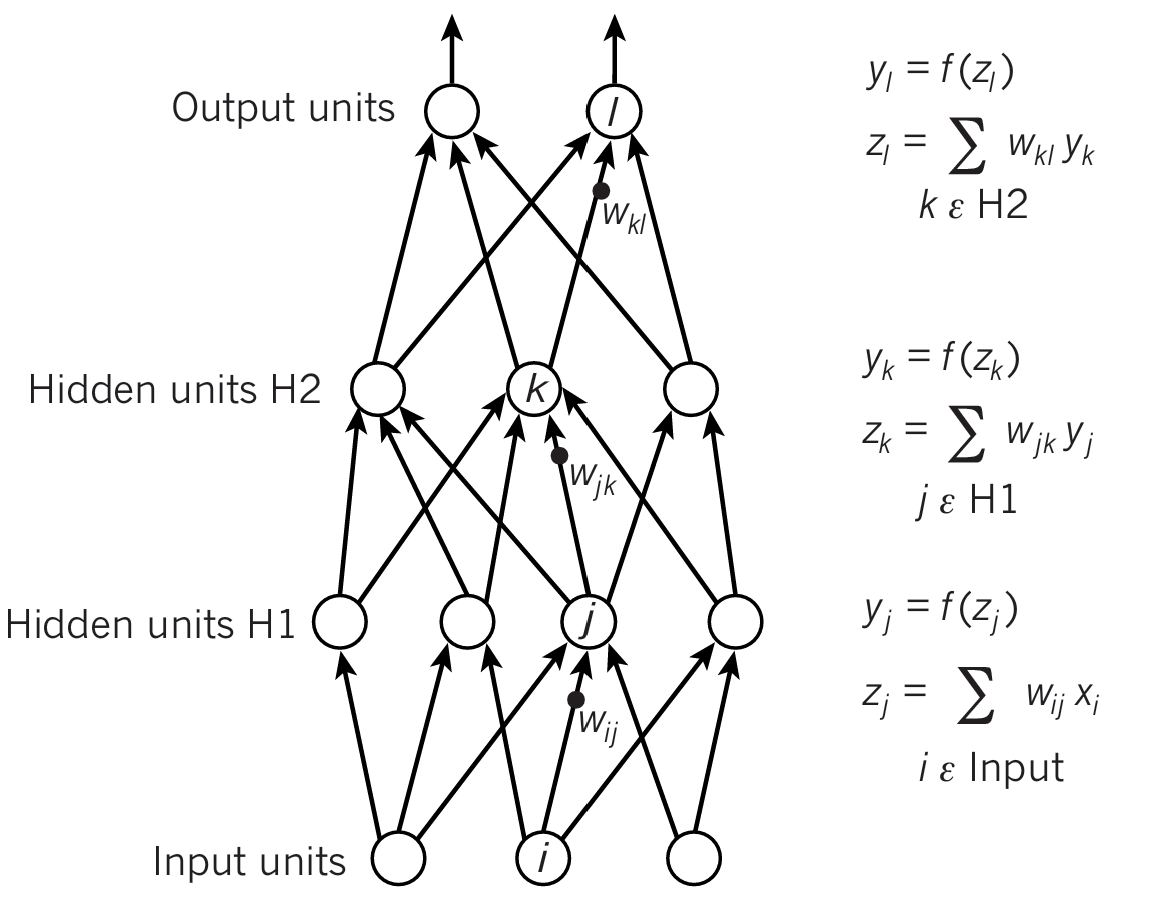
\includegraphics[scale=0.5]{/nfs/homes/sdreyer/Digit-Classification-Pytorch/tudothesis-main/content/abbildungen/Aufbau NN.png}
  \caption{Aufbau eines Neuronalen Netzwerkes.~\cite{lecun2015deep}}
  \label{fig:NN}
\end{figure}
Jedes Neuron ist dabei mit jedem aus der Vorherigen Schicht verbunden durch eine Gewichtung $w_{ij}$.
Die Aktivierung eines Neurons wird mittels einer Aktivierungsfunktion $f_\text{act}$ berechnet. In dieser fließt unter anderem die Gewichtung mit 
ein, der Eingabe Wert $x_i$ sowie ein Bias-Wert $b_i$.
\begin{equation}
    y_i = f_\text{act}\left(\sum_{i}^{n} w_{ij}x_i + b_j\right)
\end{equation}
Dieser Ausgabewert $y_i$ wird an die Neuronen in der nächsten Schicht weitergegeben.
Die meist verwendetet Aktivierungsfunktionen sind die Sigmoidfunktion, Rectifier-Funktion (ReLU-Funktion) und der hyperbolische Tangens.
Wird der Schwellenwert bei diesen Funktionen nicht erreicht, wird der Wert des Neurons nicht an die nächste Schicht weitergegeben.
Das Neuron wird inaktiv.~\cite{datascience}

\subsection{Convolutional Neural Network}

Für die Verarbeitung von Bildern eignet sich das Neuronale Netzwerk nicht, da jedes Pixel ein Eingabewert darstellt.
Aufgrund der Verbindung jedes Neurons aus der vorherigen Schicht, kommt es zu einer großen Anzahl an Verbindungen.
Durch die große Rechenkomplexität ist das Training des Netzwerkes ineffizient.
Aus diesem Grund wird gerade für die Verarbeitung von Bildern das Convolutional Neural Network (CNN) verwendet.
Bei diesem sind die Neuronen in drei Dimensionen angeordnet.
Diese sind die zwei räumlichen Dimensionen Breite und Höhe und die dritte Dimension bildet die Anzahl an Kanälen.
Das Netzwerk ist aufgebaut aus Faltungschichten (Convolutional Layers), Pooling Layers und einer Fully-Connected Layer(FC-Layer).
Zwischen den Schichten wird, wie bei den Neuronalen Netzwerken eine Aktivierungfunktion verwendet.~\cite{OShea} 
Der Aufbau eine CNN wird in der Abbildung \ref{fig:CNN} dargestellt.

\begin{figure}[htbp]
  \centering
  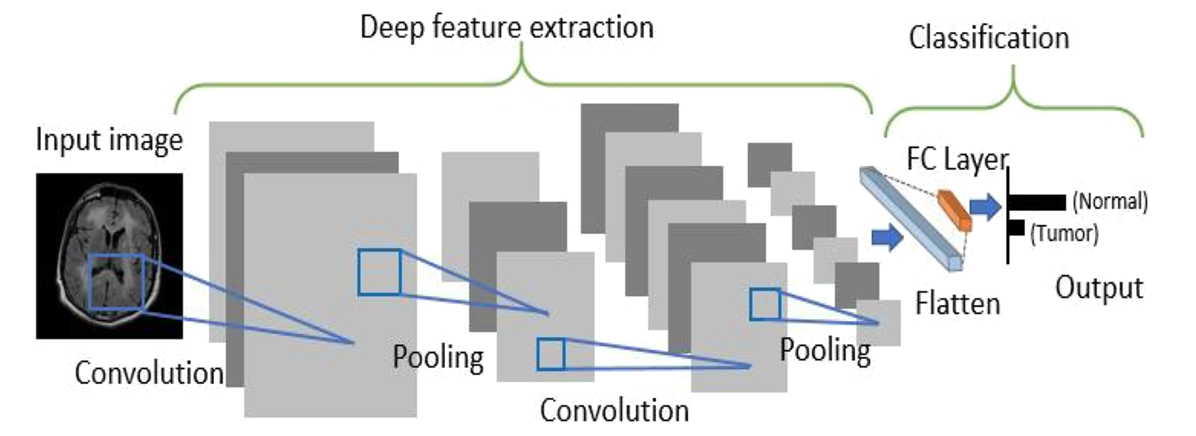
\includegraphics[scale=0.4]{/nfs/homes/sdreyer/Digit-Classification-Pytorch/tudothesis-main/content/abbildungen/CNN.png}
  \caption{Aufbau eines Convolutional Neural Network.~\cite{Mohammed2024}}
  \label{fig:CNN}
\end{figure}


Bei der Convolutional Layer, wird ein Filter (Kernel) verwendet, welcher schrittweise über das gesamte Input Bild gelegt wird.
Dieser besitzt meist eine typische Größe von $3 \times 3$, $5 \times 5$ oder $ 7 \times 7$.  
Aus dem Kernel und dem Neuron wird das Skalarprodukt berechnet, woraus eine Feature-Map erstellt wird. 
Diese Feature-Map beinhaltet die wichtigsten Strukturen.
Damit der Filter auch den Rand des Bildes mit dem Zentrum überlappen kann, wird das sogenannte Padding angewendet.
Beim Zero-padding, wird am Rand des Bildes Nullen hinzugefügt. Dadurch bleibt die räumliche Dimension erhalten.
Als Stride wird der Abstand zwischen zwei Positionen des Kernels beschrieben. Am häufigsten wird ein stride von 1 gewählt. 
Das bedeutet, dass nach jeder Berechnung des Skalarproduktes der Kernel um eine Position verschiebt.
\begin{figure}[htbp]
  \centering
  \begin{subfigure}[b]{0.3\textwidth}
    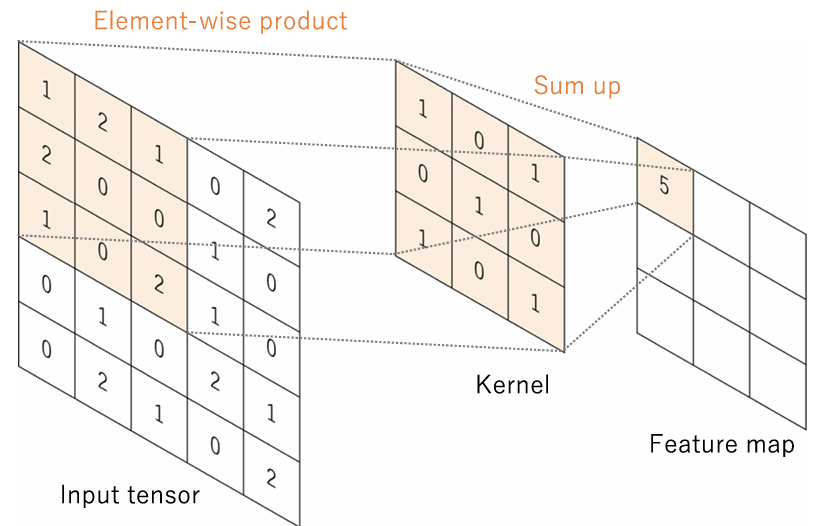
\includegraphics[width=\textwidth]{/nfs/homes/sdreyer/Digit-Classification-Pytorch/tudothesis-main/content/abbildungen/kernel a.png}
    %\caption{}
    \label{}
  \end{subfigure}
  \hfill
  \begin{subfigure}[b]{0.3\textwidth}
    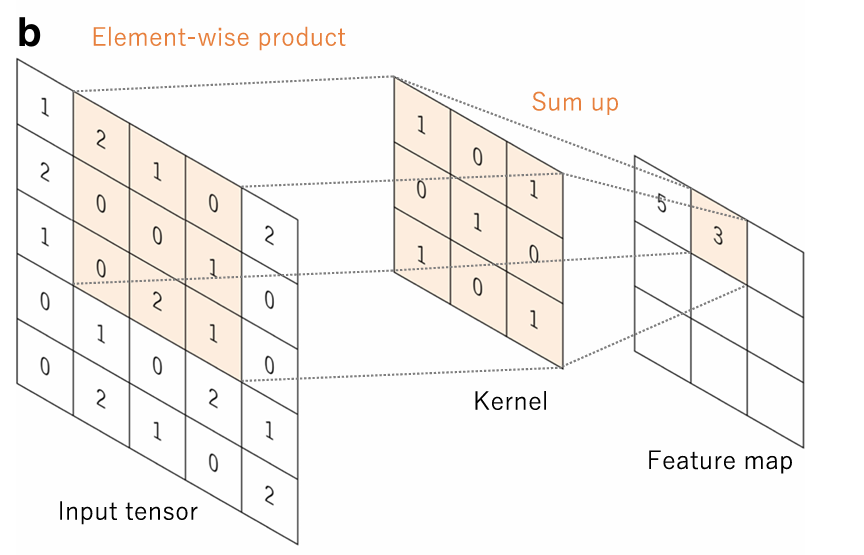
\includegraphics[width=\textwidth]{/nfs/homes/sdreyer/Digit-Classification-Pytorch/tudothesis-main/content/abbildungen/kernel b.png}
    %\caption{}
    \label{}
  \end{subfigure}
  \hfill
  \begin{subfigure}[b]{0.3\textwidth}
    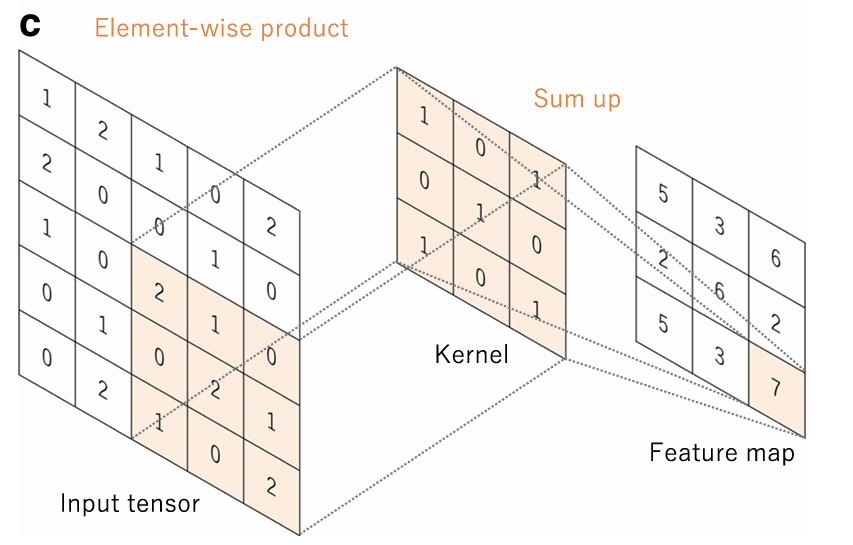
\includegraphics[width=\textwidth]{/nfs/homes/sdreyer/Digit-Classification-Pytorch/tudothesis-main/content/abbildungen/kernel c.png}
    %\caption{}
    \label{}
  \end{subfigure}
  \caption{Ein Beispiel der Convolutional layer mit der Verwendung eines Kernels der Größe $3 \times 3$.~\cite{Yamashita2018}}
  \label{fig:kernel}
\end{figure}

Die Pooling-Layer reduziert die räumliche Dimension. Infolge dessen kommt es auch zur Reduktion der Parameter der Aktivierung.~\cite{datascience}
Dafür wird das sogenannte Max-Pooling verwendet. Dabei wirf ein Filter der Größe $2 \times 2$ verwendet, der wie der Kernel, schrittweise über die Feature-Map gelegt wird.
Für jeden Ausschnitt wird der größte Wert verwendet. Der Rest der Werte wird nicht weiter verwendet.~\cite{Yamashita2018}\\

Die FC-Layer berechnet am Ende die Aktivierung und bestimmt einen Ausgangswert für die Klassifizierung.


